\documentclass{beamer}
\usepackage[latin1]{inputenc}
\usepackage{times}
\usepackage{tikz}
\usetheme{Luebeck}
%\usecolortheme{albatross}
\usepackage{amsmath,amsfonts,amsthm,amssymb}
\usepackage{setspace}
\usepackage{Tabbing}
\usepackage{fancyhdr}
\usepackage{lastpage}
\usepackage{extramarks}
\usepackage{chngpage}
\usepackage{soul,color}
\usepackage{graphicx,float,wrapfig}
\usepackage{xcolor}
\usepackage{listings}
\usepackage{float}
%\usepackage{subfloat}
\usepackage{subfig}
\usepackage{caption}
\usepackage{enumitem}
\usepackage{algpseudocode}

\definecolor{darkorange}{RGB}{240, 120, 0}
\definecolor{darkgreen}{RGB}{0, 128, 0}

\setbeamercolor{background canvas}{bg=white}
\setbeamercolor{frametitle}{fg=white, bg=darkorange}
\setbeamercolor{normal text}{bg=black,fg=black}
\setbeamercolor{structure}{bg=black, fg=darkorange}


\lstdefinestyle{customc}{
  belowcaptionskip=1\baselineskip,
  breaklines=true,
  frame=L,
  xleftmargin=\parindent,
  language=Python,
  showstringspaces=false,
  basicstyle=\footnotesize\ttfamily,
  keywordstyle=\bfseries\color{green!40!black},
  commentstyle=\itshape\color{purple!40!black},
  identifierstyle=\color{blue},
  stringstyle=\color{orange},
}

\lstdefinestyle{customc}{
  belowcaptionskip=1\baselineskip,
  breaklines=true,
  frame=L,
  xleftmargin=\parindent,
  language=Python,
  showstringspaces=false,
  basicstyle=\footnotesize\ttfamily,
  keywordstyle=\bfseries\color{green!40!black},
  commentstyle=\itshape\color{purple!40!black},
  identifierstyle=\color{blue},
  stringstyle=\color{orange},
}

\lstdefinestyle{customcsmall}{
  belowcaptionskip=1\baselineskip,
  breaklines=true,
  frame=L,
  xleftmargin=\parindent,
  language=Python,
  showstringspaces=false,
  basicstyle=\footnotesize\ttfamily,
  keywordstyle=\bfseries\color{green!24!black},
  commentstyle=\itshape\color{purple!24!black},
  identifierstyle=\color{blue},
  stringstyle=\color{orange},
}

\lstdefinestyle{customcsmall}{
  belowcaptionskip=1\baselineskip,
  breaklines=true,
  frame=L,
  xleftmargin=\parindent,
  language=Python,
  showstringspaces=false,
  basicstyle=\footnotesize\ttfamily,
  keywordstyle=\bfseries\color{green!24!black},
  commentstyle=\itshape\color{purple!24!black},
  identifierstyle=\color{blue},
  stringstyle=\color{orange},
}

\definecolor{MidGreen}{HTML}{00AA00}
\definecolor{MidYellow}{HTML}{AAAA00}

\title{Lecture 18: Fourier Decomposition, Circular Functions, Spherical Harmonics}
\date{3/22/2016}
\institute{Chris Tralie, Duke University}
\author{COMPSCI/MATH 290-04}
\begin{document}

\frame{\titlepage}

\begin{frame}{Announcements}
\begin{itemize}[label=$\vartriangleright$]

\item Midterms graded
\uncover<2-> {
\item Group Assignment 1 Graded, Art contest up online (great work!!)
}

\uncover<3->{
\item Group Assignment 2 Due Wednesday 3/30

\item Piazza hours 8-9PM week nights (student Piazza answers encouraged)
}

\uncover<4-> {
\item T.A.s grading mini assignment 3

}

\uncover<5->{
\item No more extra credit for now
}

\uncover<6->{
\item Final project directions sent out, first milestone due Friday 4/8

\item Ditching Wikipedia entry, final project now worth 30 \%
}

\end{itemize}

\end{frame}

\begin{frame}{Table of Contents}
\begin{itemize}[label=$\blacktriangleright$]
	\item 1D Fourier Decomposition / Circle Functions
\end{itemize}
\begin{itemize}[label=$\vartriangleright$]
	\item 2D Fourier Modes
\end{itemize}
\begin{itemize}[label=$\vartriangleright$]
	\item Spherical Harmonics
\end{itemize}
\end{frame}

\begin{frame}{Why Fourier?? (Interlude)}

Hey Chris, isn't this a course on 3D geometry??  Why Fourier???

\begin{itemize}[label=$\vartriangleright$]
\uncover<2->{
\item Most CS majors don't know about it, but {\em extremely important}
}

\uncover<3->{
\item Picks up on ``shape" in a different way
}

\uncover<4->{
\item Entry point into harmonic analysis, nonrigid surface statistics
}
\end{itemize}

\end{frame}

\begin{frame}{Sinusoid Review}

\[ f(x) = A \cos( \omega x + \phi) \]

\[ f(x) = (A\cos(\phi))\textcolor{red}{\cos(\omega x)} - (A\sin(\phi))\textcolor{blue}{\sin(\omega x)} \]

\uncover<2->{

\[ f(x) =  a \cos(\omega x) + b \sin(\omega x) \]

\[ A = \sqrt{a^2 + b^2}, \phi = \tan^{-1}(\frac{b}{a}) \]

}

\uncover<3->{

In {\em polar form}

\[ f(x) = Ae^{i (\omega x + \phi)} = A e^{i \phi} e^{i \omega x} = A (\cos(\theta) + i \sin(\theta)) e^{i \omega x} \]

}

\end{frame}

\begin{frame}{Sinusoid Example}

\begin{figure}[t]
    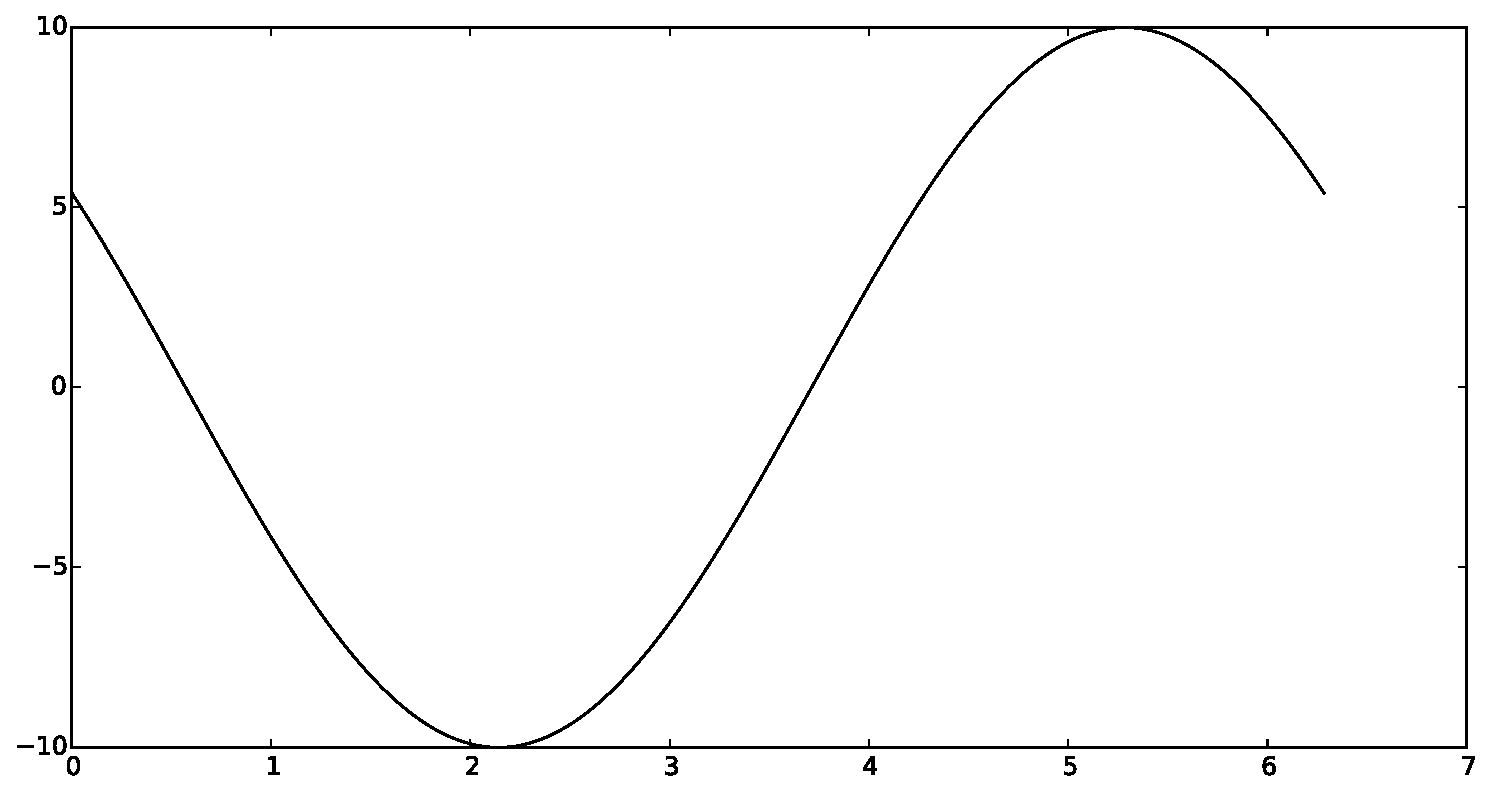
\includegraphics[width=\textwidth]{SineDecomp1.pdf}
\end{figure}

\end{frame}

\begin{frame}{Sinusoid Example}

\begin{figure}[t]
    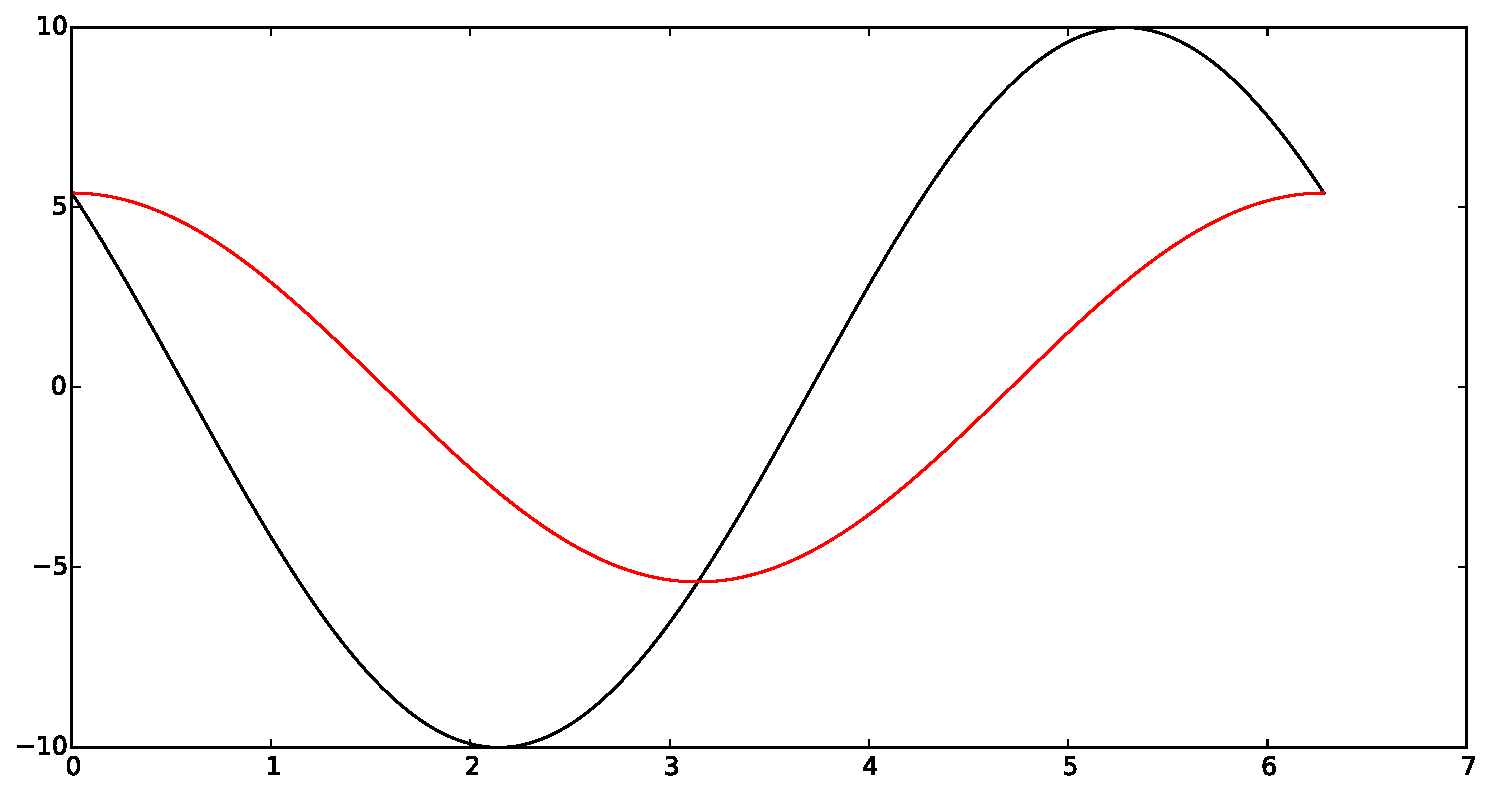
\includegraphics[width=\textwidth]{SineDecomp2.pdf}
\end{figure}

\end{frame}

\begin{frame}{Sinusoid Example}

\begin{figure}[t]
    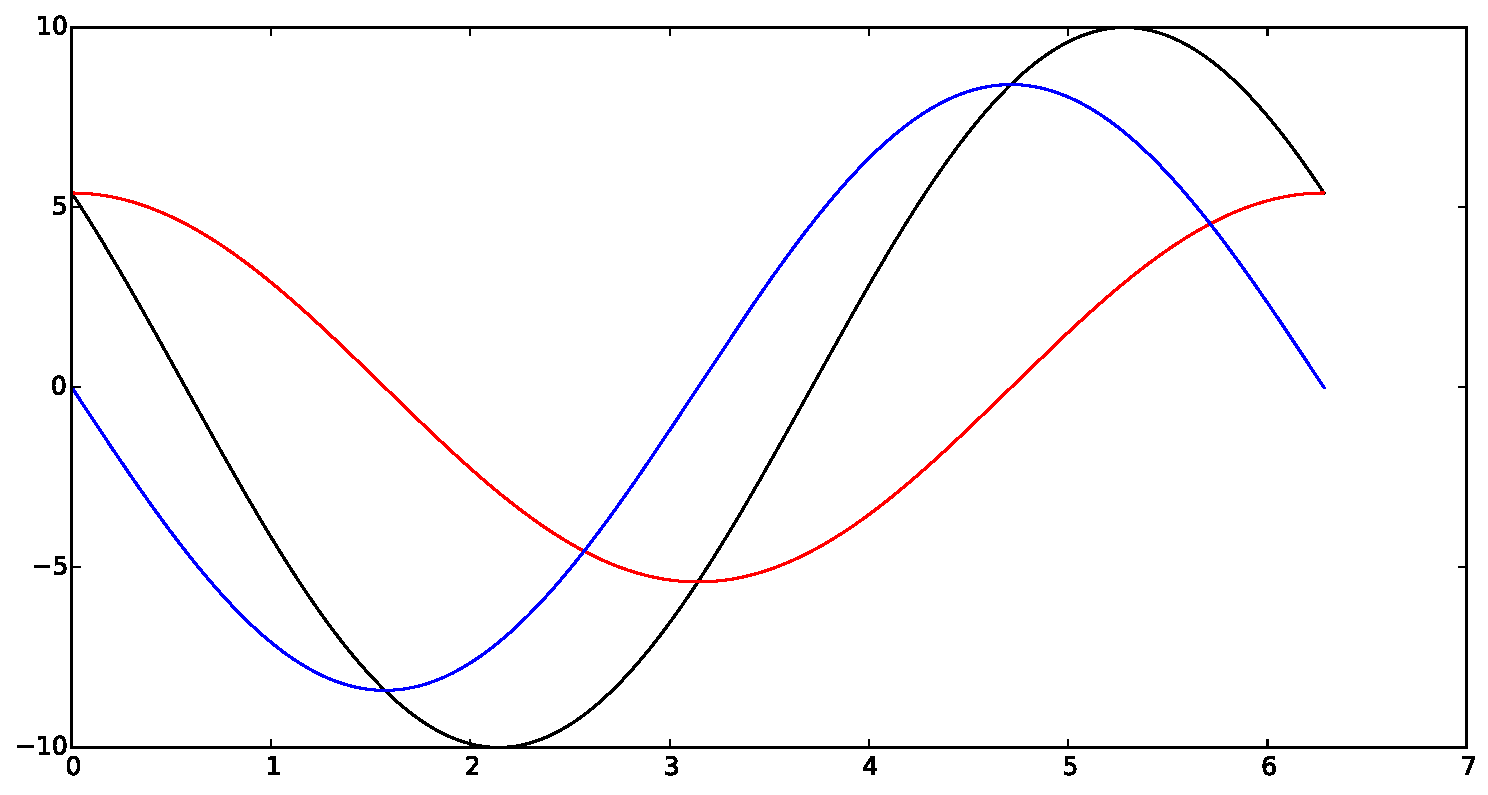
\includegraphics[width=\textwidth]{SineDecomp3.pdf}
\end{figure}

\end{frame}

\begin{frame}{Fourier Decomposition}

\begin{figure}[t]
    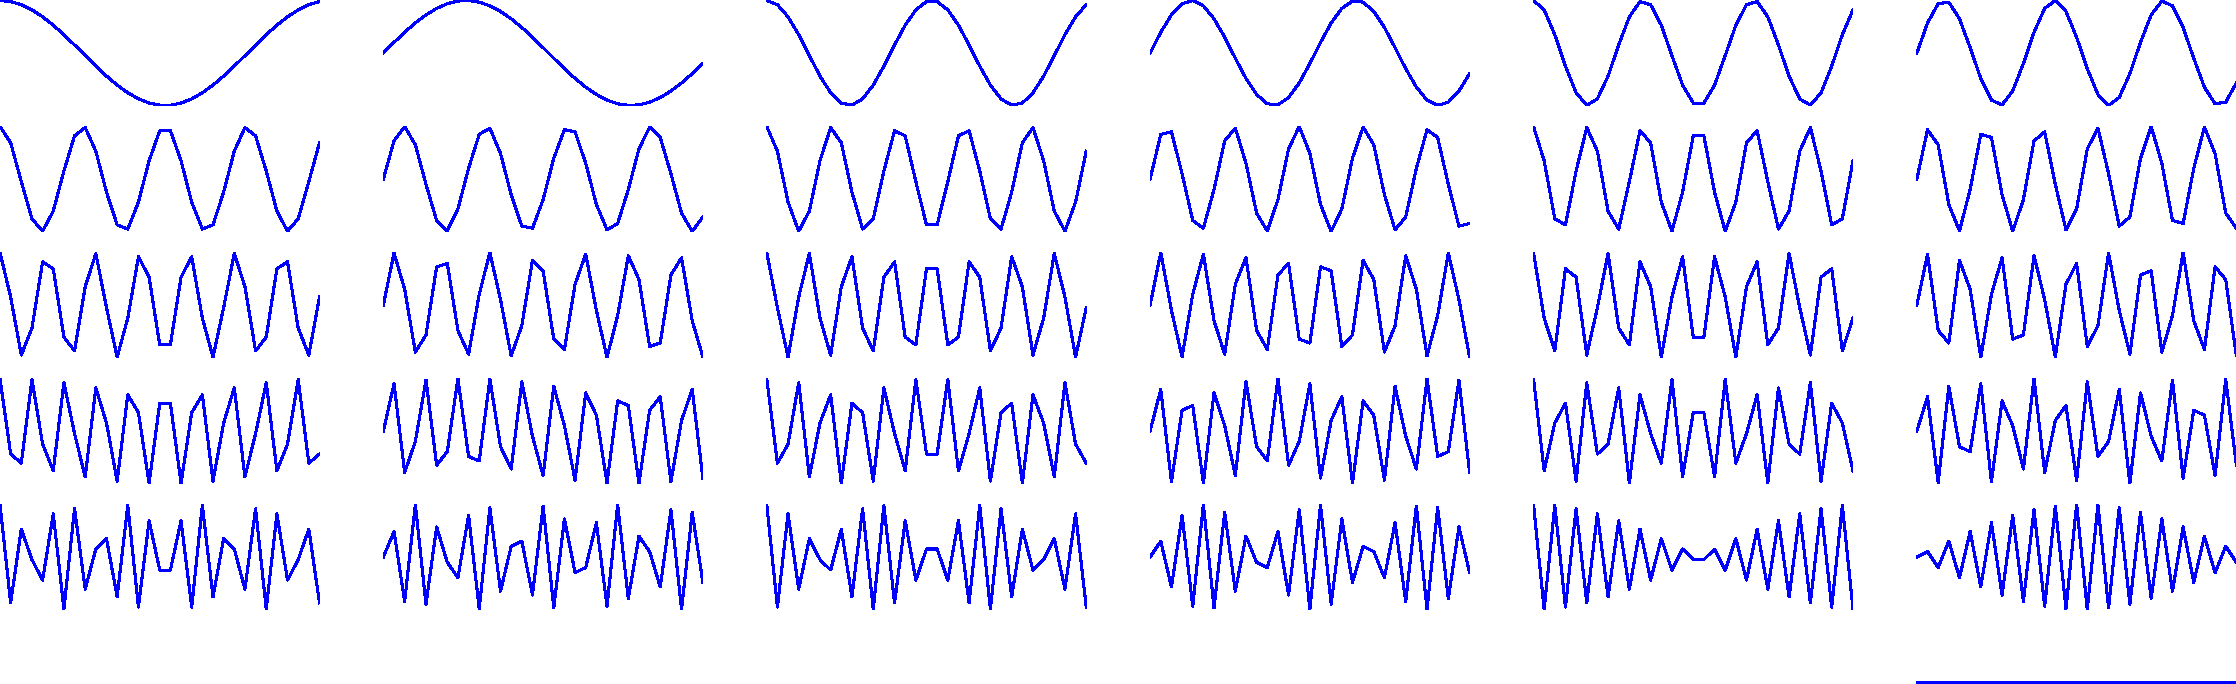
\includegraphics[width=\textwidth]{FourierBasis.pdf}
\end{figure}

\[ f[n] = \sum_{k = 0}^{N-1} a_k \cos \left( \frac{2\pi k}{N} n \right) + b_k \sin \left( \frac{2\pi k}{N} n \right) \]

Amplitude at frequency index $k$ is $\sqrt{a_k^2 + b_k^2}$

\end{frame}



\begin{frame}{Fourier Decomposition: Gaussian Examples}

Show video frames

\end{frame}


\begin{frame}{Fourier Decomposition: Gaussian Examples}

\begin{figure}[t]
    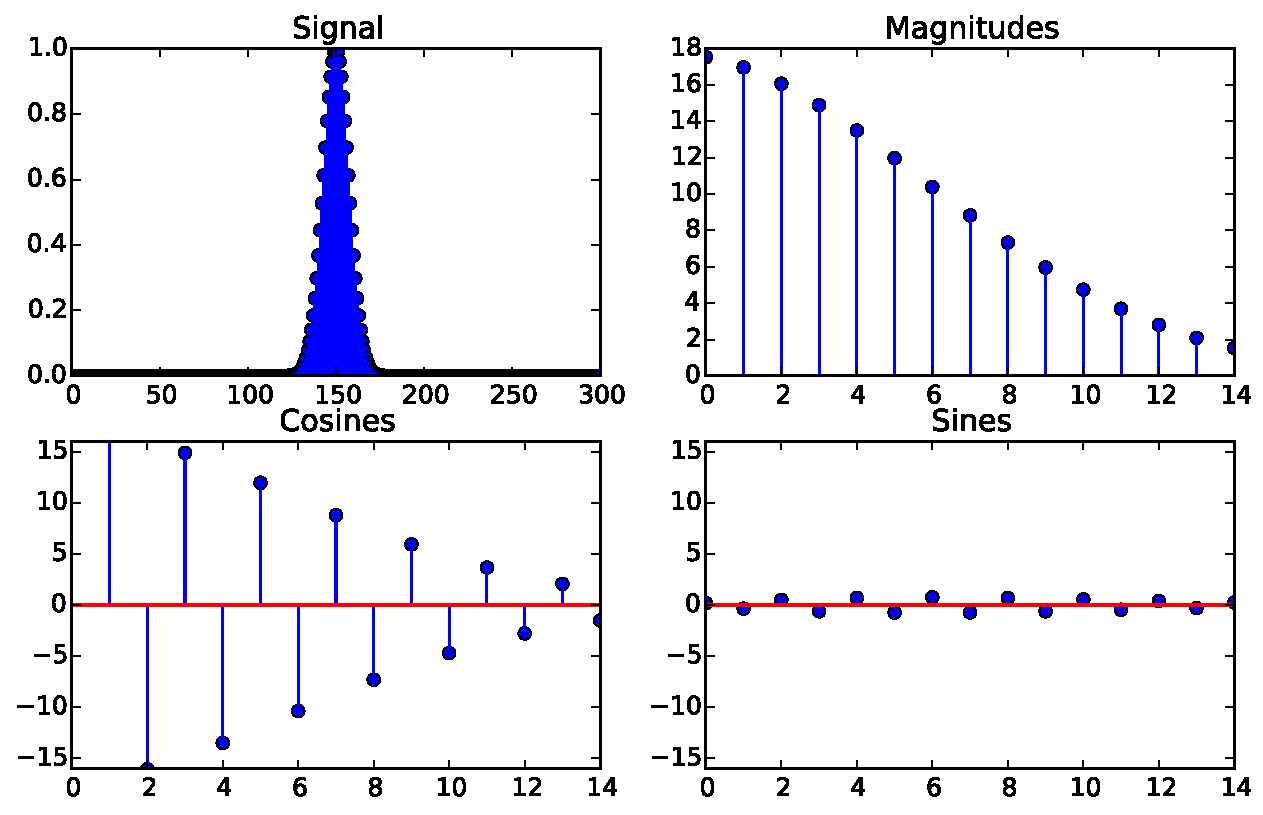
\includegraphics[width=\textwidth]{GaussSig10_1/SignalDecomposition.pdf}
\end{figure}

\end{frame}

\begin{frame}{Fourier Decomposition: Gaussian Examples}

\begin{figure}[t]
    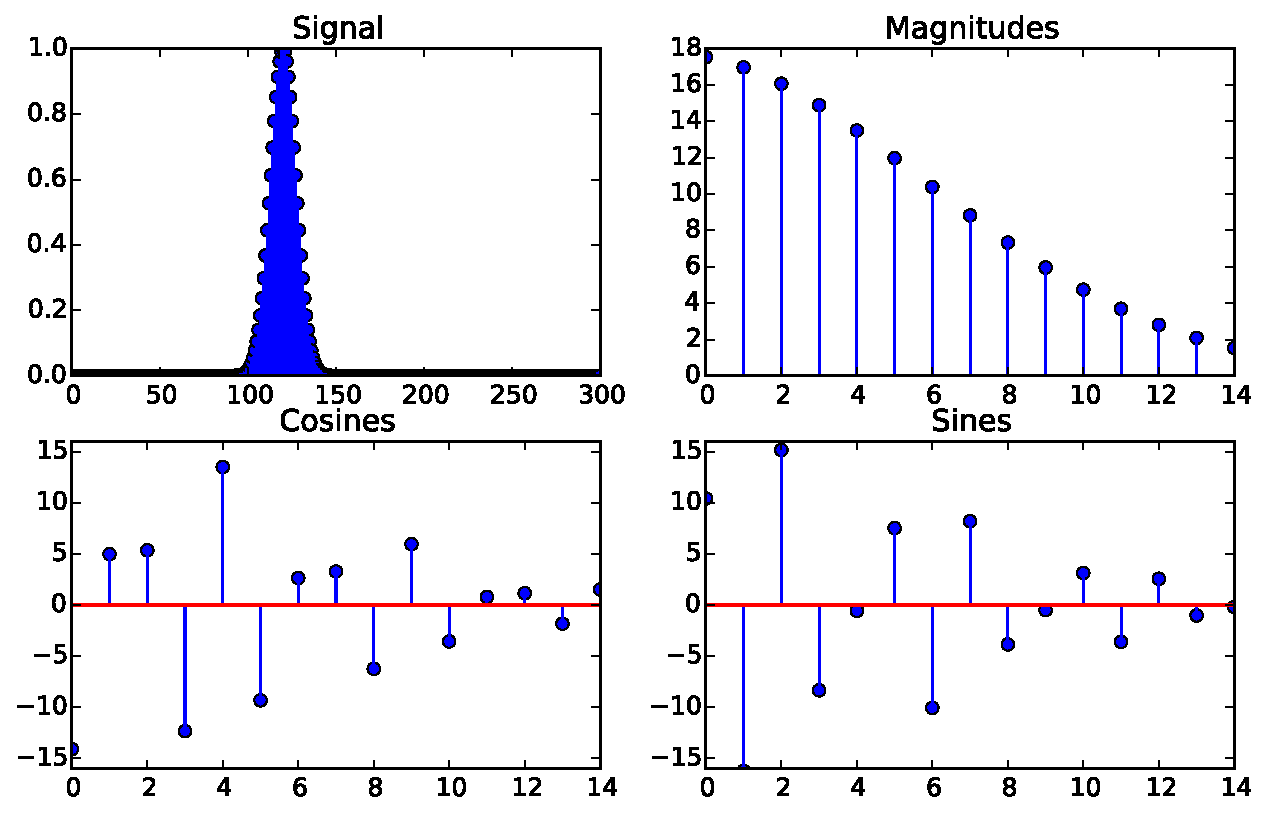
\includegraphics[width=\textwidth]{GaussSig10_2/SignalDecomposition.pdf}
\end{figure}

\end{frame}


\begin{frame}{Fourier Decomposition: Ramp Example}

Show video frames

\end{frame}

\begin{frame}{Fourier Decomposition: Ramp Example}

\begin{figure}[t]
    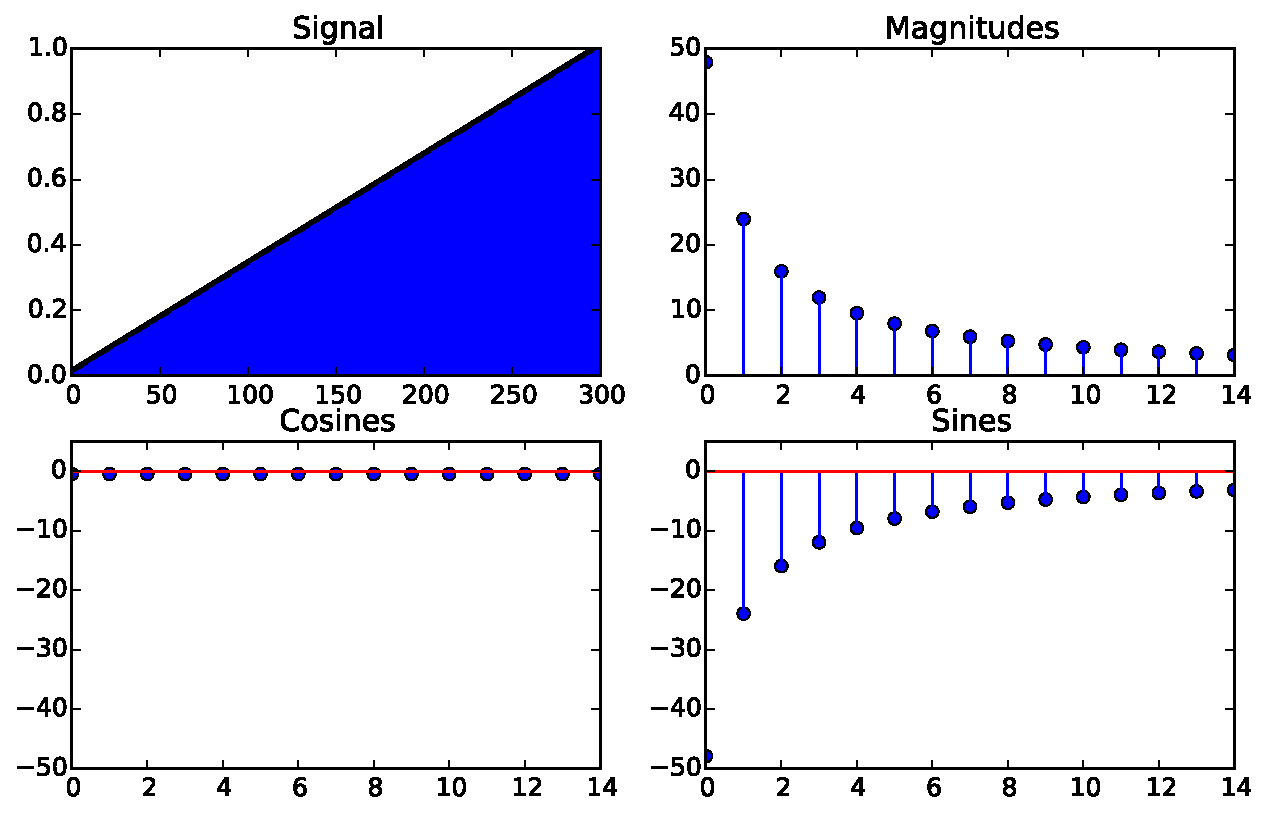
\includegraphics[width=\textwidth]{Ramp1/SignalDecomposition.pdf}
\end{figure}

\end{frame}

\begin{frame}{Fourier Decomposition: Ramp Example}

\begin{figure}[t]
    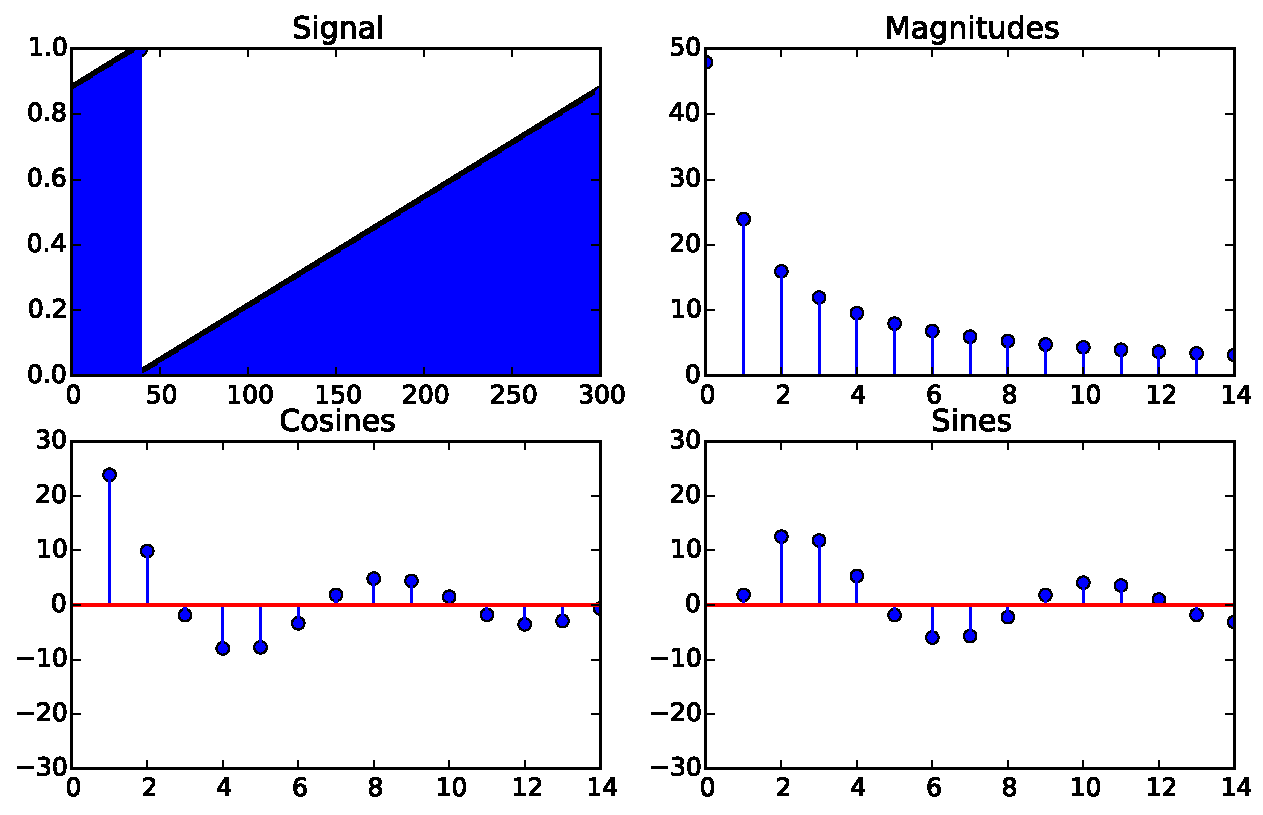
\includegraphics[width=\textwidth]{Ramp2/SignalDecomposition.pdf}
\end{figure}

\end{frame}

\begin{frame}{Fourier Decomposition: Ramp Example}

\begin{figure}[t]
    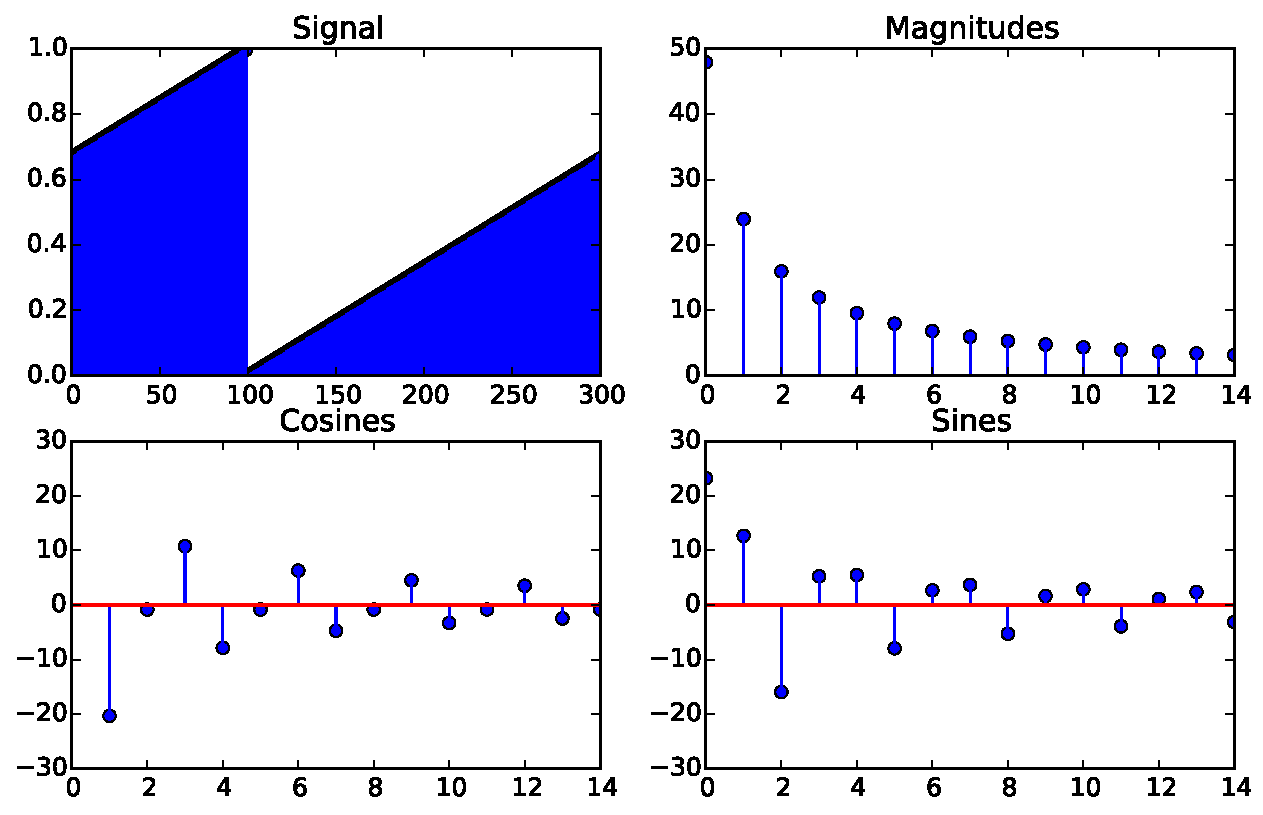
\includegraphics[width=\textwidth]{Ramp3/SignalDecomposition.pdf}
\end{figure}

\end{frame}

\begin{frame}{Fourier Decomposition: Ramp Example}

Continuous shifting videos

\end{frame}


\begin{frame}{Functions on The Circle}

\begin{figure}
    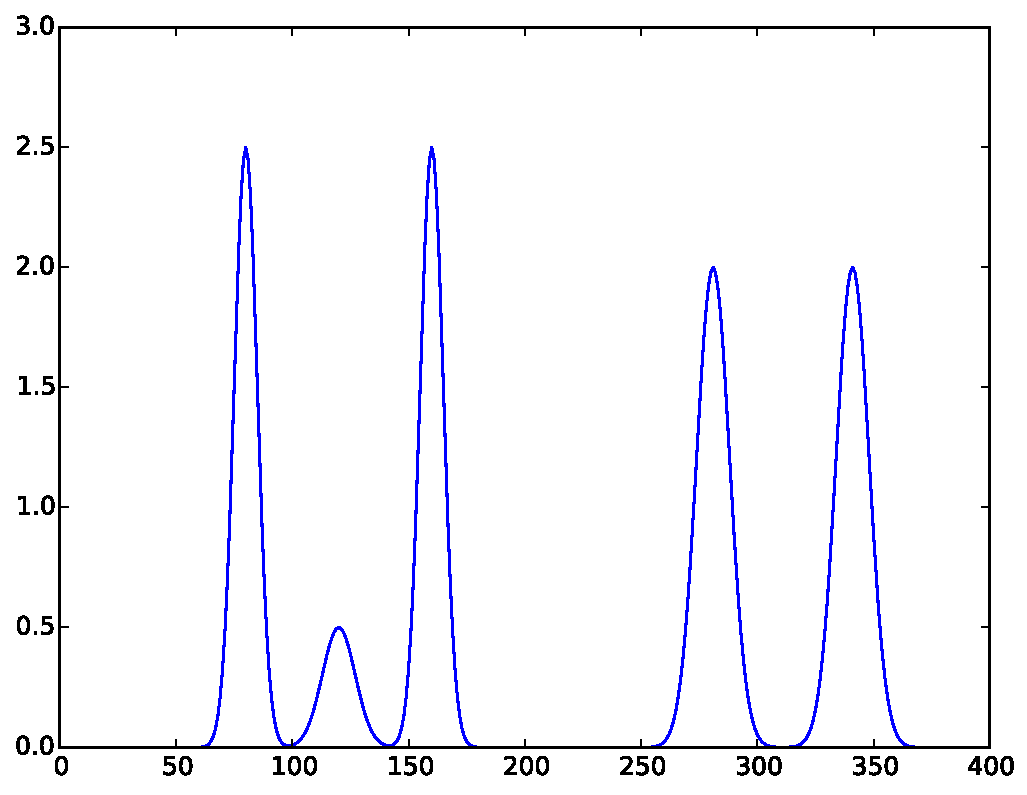
\includegraphics[width=0.8\textwidth]{5Gaussians.pdf}
\end{figure}

Show circle wrap video

\end{frame}


\begin{frame}{Functions on The Circle}

\begin{figure}
    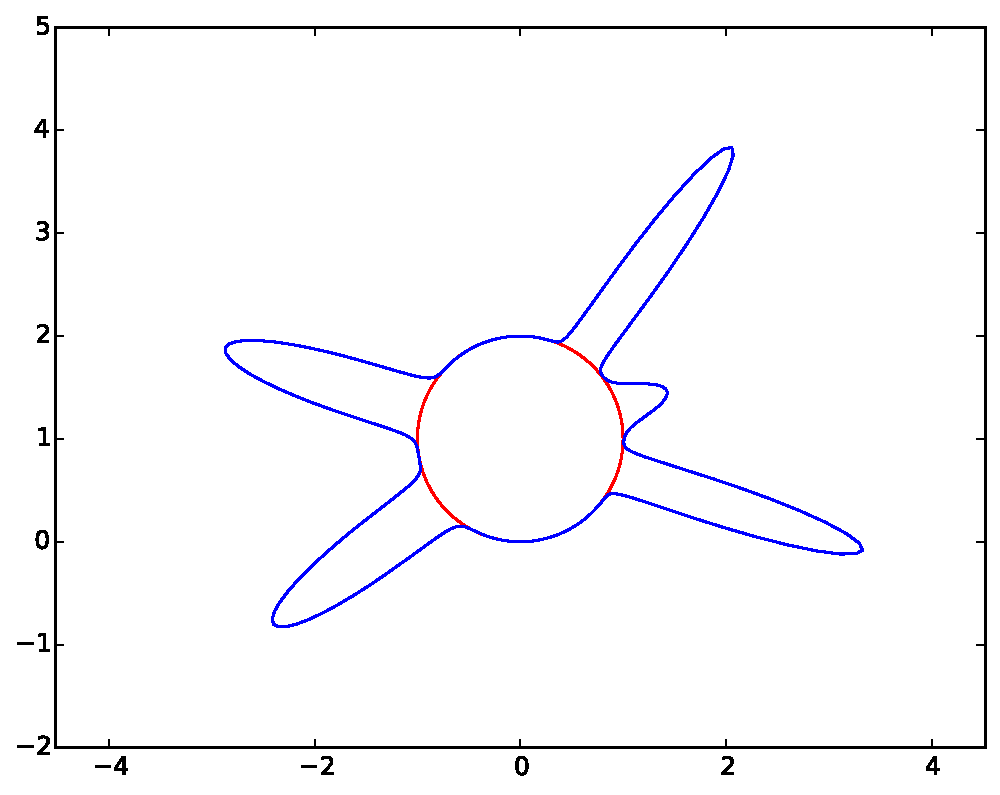
\includegraphics[width=0.8\textwidth]{5GaussiansCircleWrap.pdf}
\end{figure}


\end{frame}

\begin{frame}

Phase as a rotation

\[ g(x) = f(x + \phi) \]

Show video

\end{frame}


\begin{frame}{Table of Contents}
\begin{itemize}[label=$\vartriangleright$]
	\item 1D Fourier Decomposition / Circle Functions
\end{itemize}
\begin{itemize}[label=$\blacktriangleright$]
	\item 2D Fourier Modes
\end{itemize}
\begin{itemize}[label=$\vartriangleright$]
	\item Spherical Harmonics
\end{itemize}
\end{frame}


\begin{frame}{2D Sinusoids (aka ``Plane Waves")}

\[ f(x, y) = \cos( \omega_x x + \omega_y y + \phi) \]

\[ f(x, y) = \cos( \vec{\omega} \cdot \vec{x} + \phi ) \]

\end{frame}


\begin{frame}{2D Sinusoids: Example}

\[ f(x, y) = \cos( x + y ), \omega_x = 1, \omega_y = 1 \]

\begin{figure}[t]
    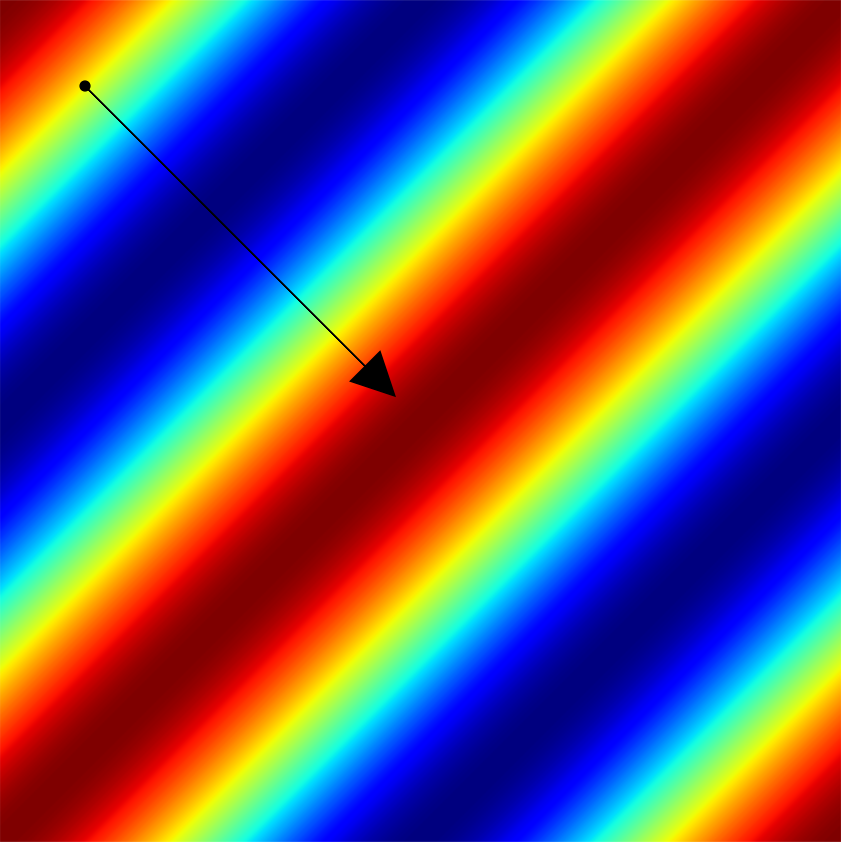
\includegraphics[width=0.6\textwidth]{2DPlaneWaves/1_1.png}
\end{figure}

\end{frame}



\begin{frame}{2D Sinusoids: Example}

\[ f(x, y) = \cos( 2x + 2y ), \omega_x = 2, \omega_y = 2 \]

\begin{figure}[t]
    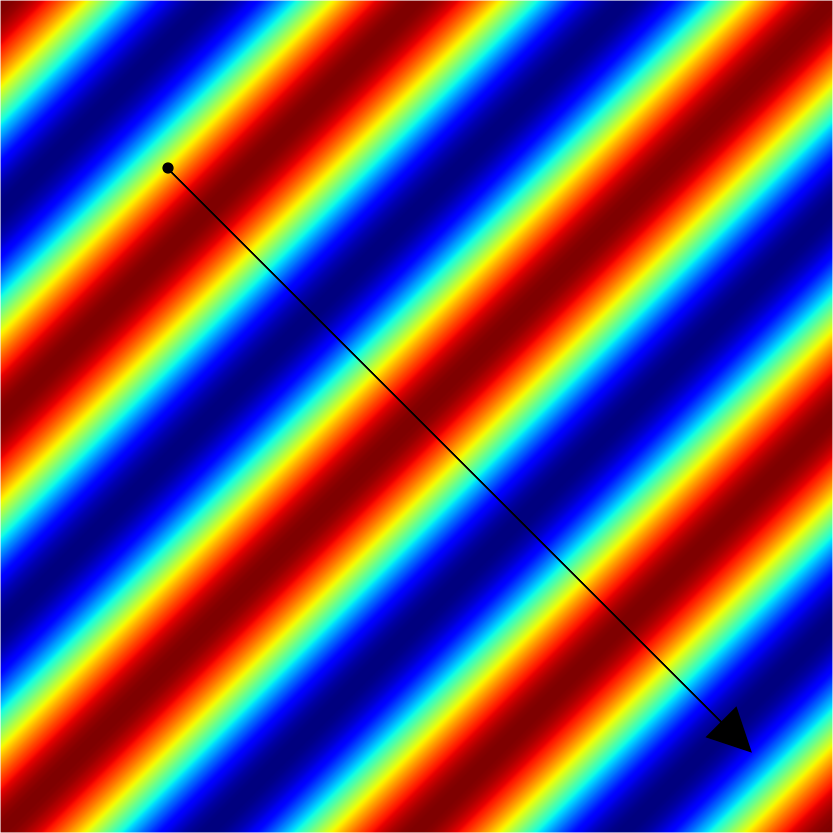
\includegraphics[width=0.6\textwidth]{2DPlaneWaves/2_2.png}
\end{figure}

\end{frame}


\begin{frame}{2D Sinusoids: Example}

\[ f(x, y) = \cos( x + 2y ), \omega_x = 1, \omega_y = 2 \]

\begin{figure}[t]
    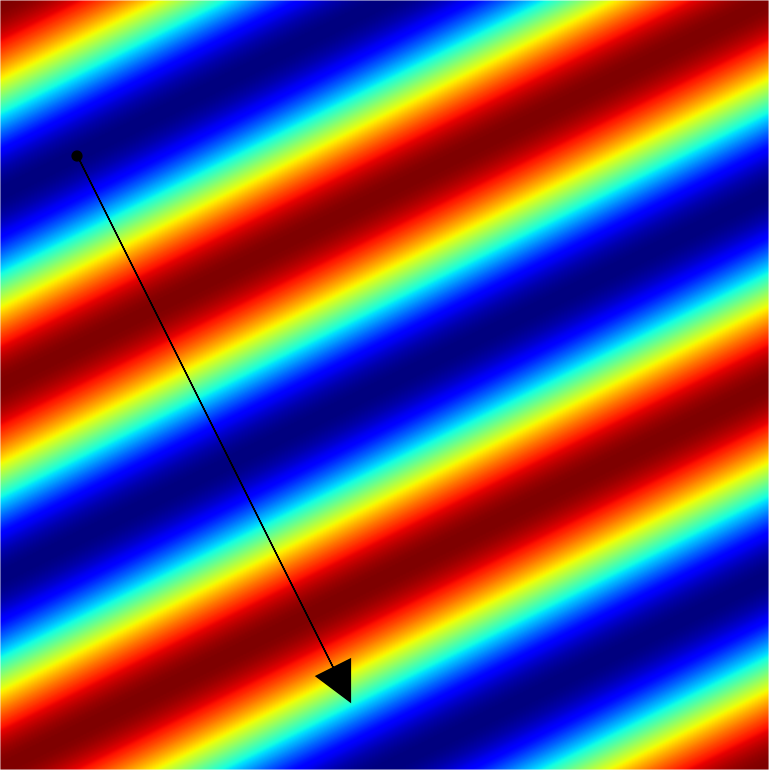
\includegraphics[width=0.6\textwidth]{2DPlaneWaves/1_2.png}
\end{figure}

\end{frame}



\begin{frame}{2D Sinusoids: Example}

\[ f(x, y) = \cos( x ), \omega_x = 1, \omega_y = 0 \]

\begin{figure}[t]
    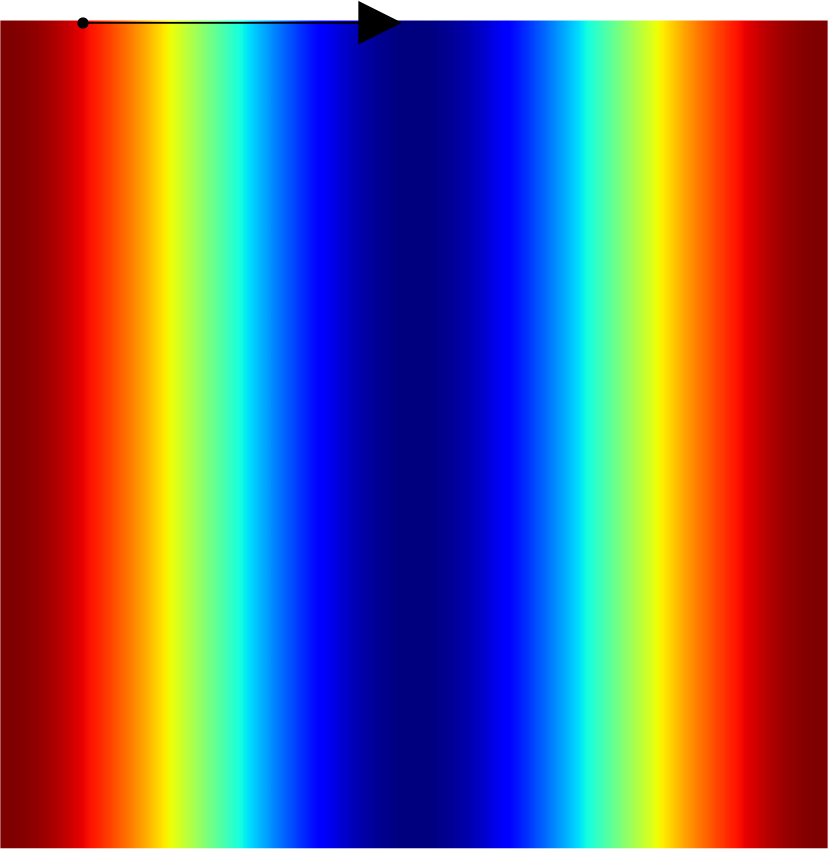
\includegraphics[width=0.6\textwidth]{2DPlaneWaves/1_0.png}
\end{figure}

\end{frame}


\begin{frame}{2D Sinusoids: Example}

\[ f(x, y) = \cos( 1.5y ), \omega_x = 0, \omega_y = 1.5 \]

\begin{figure}[t]
    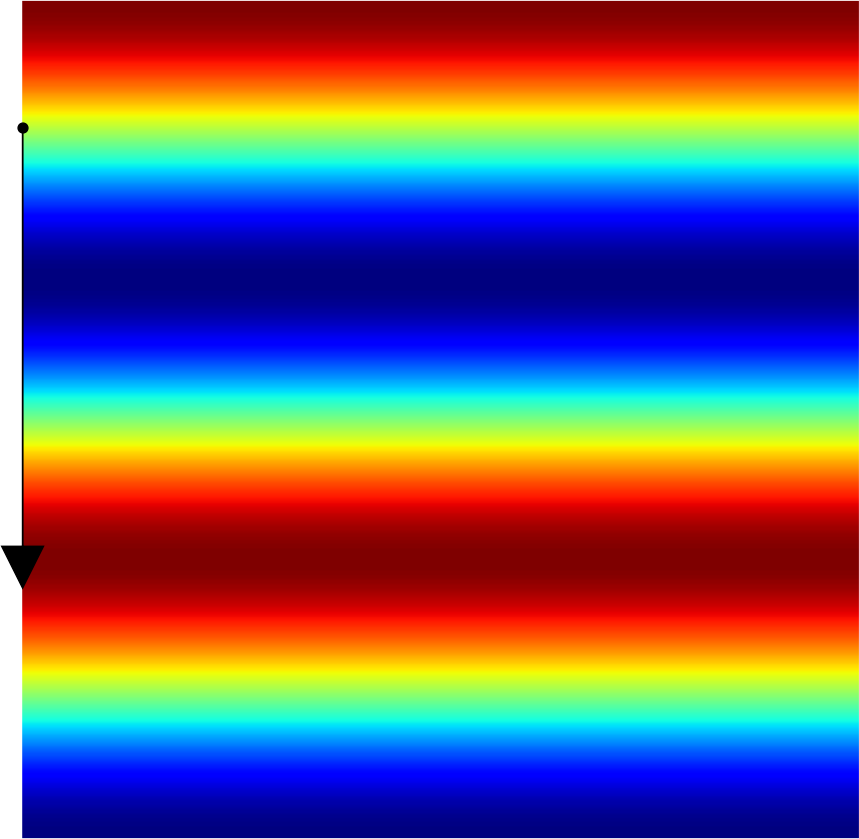
\includegraphics[width=0.6\textwidth]{2DPlaneWaves/0_1pt5.png}
\end{figure}

\end{frame}


\begin{frame}{2D Sinusoids: Interference Pattern}

\[ f(x, y) = \cos(x + y) + \cos(x - y) \]

\begin{figure}[t]
    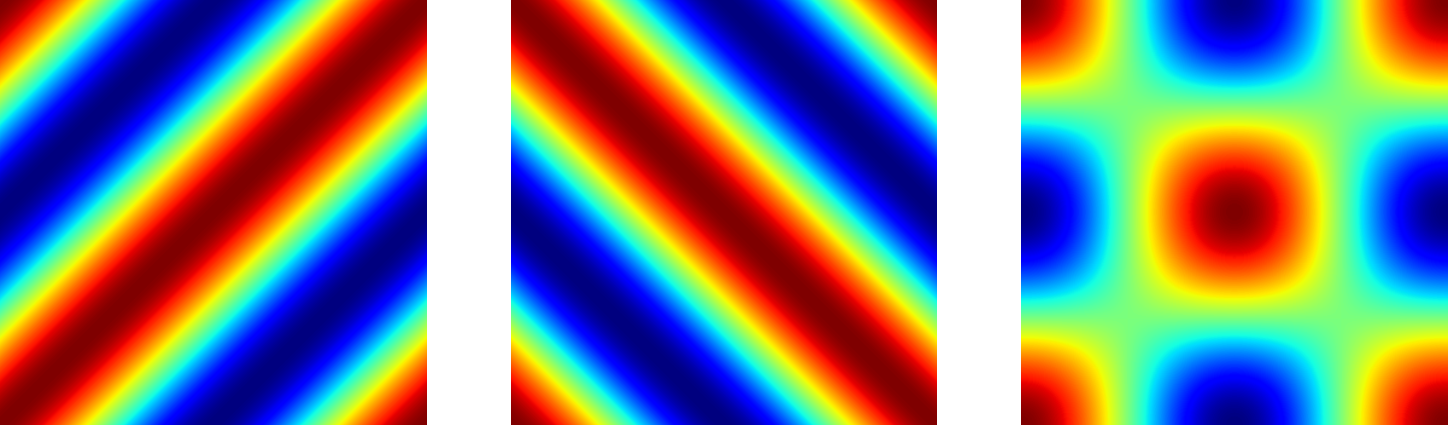
\includegraphics[width=\textwidth]{2DInterference/Interference_11.png}
\end{figure}


\end{frame}

\begin{frame}{2D Sinusoids: Interference Pattern}

\[ f(x, y) = \cos(2x + y) + \cos(2x - y) \]

\begin{figure}[t]
    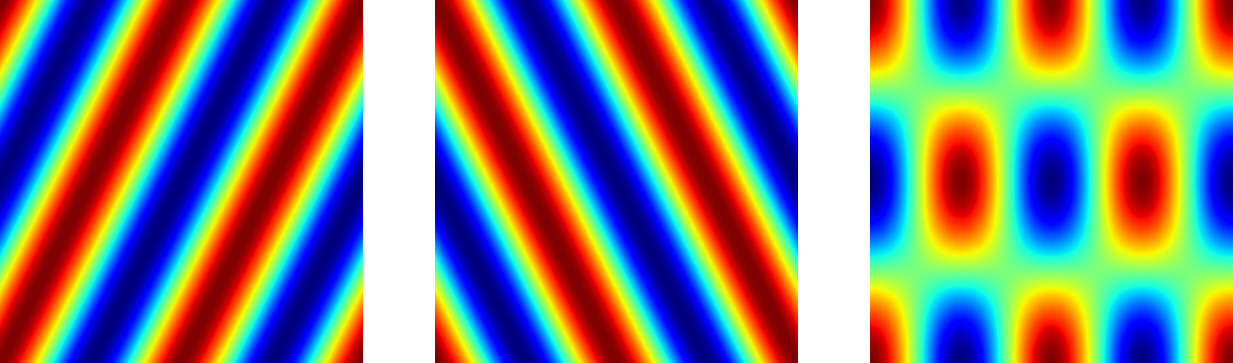
\includegraphics[width=\textwidth]{2DInterference/Interference_21.png}
\end{figure}


\end{frame}



\begin{frame}{2D Sinusoids: Interference Pattern}

\[ f(x, y) = \cos(3x + 2y) + \cos(3x - 2y) \]

\begin{figure}[t]
    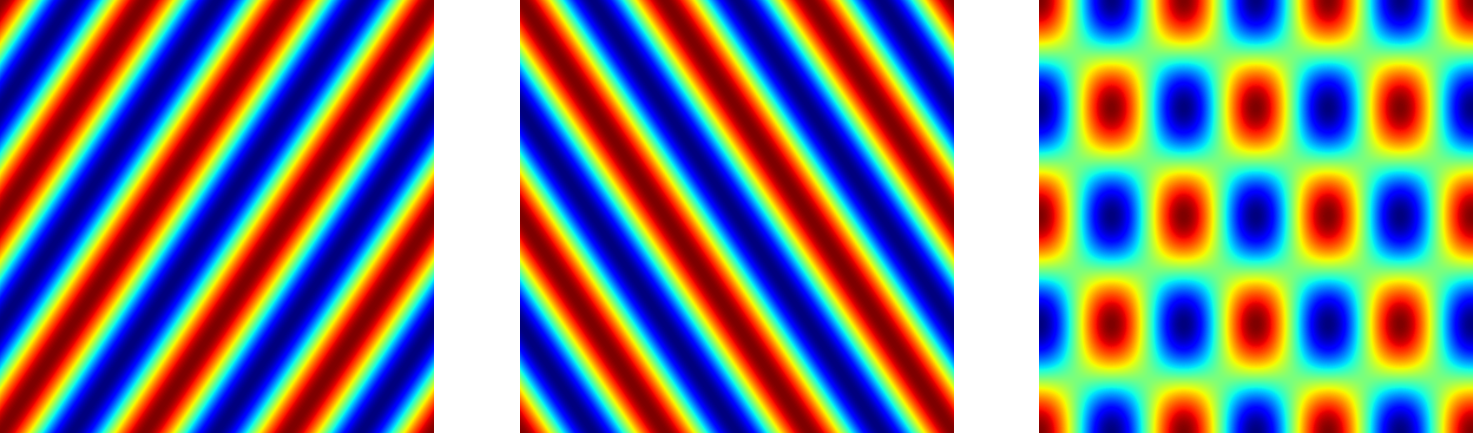
\includegraphics[width=\textwidth]{2DInterference/Interference_32.png}
\end{figure}


\end{frame}


\begin{frame}{2D Sinusoids: Interference}

Why is this happening?

\[ g(x, y) = \cos(\omega_x x + \omega_y y) + \cos(\omega_x x - \omega_y y) \]

\uncover<2-> {
    \[ g(x, y) = \cos(\omega_x x)\cos(\omega_y y) - \sin(\omega_x x)\sin(\omega_y y) \] 
    \[+ \cos(\omega_x x)\cos(\omega_y y) + \sin(\omega_x x)\sin(\omega_y y) \]
}

\uncover<3-> {
    \[ g(x, y) = 2 \cos(\omega_x x)\cos(\omega_y y) \]
}

\end{frame}


\begin{frame}{Table of Contents}
\begin{itemize}[label=$\vartriangleright$]
	\item 1D Fourier Decomposition / Circle Functions
\end{itemize}
\begin{itemize}[label=$\vartriangleright$]
	\item 2D Fourier Modes
\end{itemize}
\begin{itemize}[label=$\blacktriangleright$]
	\item Spherical Harmonics
\end{itemize}
\end{frame}


\begin{frame}{Spherical Coordinates Review}


\end{frame}


\begin{frame}{Spherical Harmonics}

%\[ Y^m_l (\theta, \phi) = \sqrt{ \frac{(2m+1){4 \pi}} \frac{(m - |n|)!}{(m + |n|)!}} P_

\[ Y^m_l \propto P_{l}^m(\cos(\theta)) e^{i m \phi} \]

Interactive Demo

\end{frame}


\begin{frame}{Spherical Harmonic Shape Descriptors}


Show Tom's paper

\end{frame}

\end{document}

